\chapter{UMS Process Evaluation}\label{sec:processval}
	\section{Introduction}
		The system design motivated in \autoref{chap:sysdes} is chosen as the design most likely to meet the target specifications (\autoref{app:specs}). As UMS is the foundry service that the chip is designed for, a lot of the input data for the system design is based on empirical knowledge from earlier designs with the same foundry. UMS does however have several processes to choose from. Of interest are the PH25 (low noise pHEMT; \unit[0.25]{\mum} gate length) and PPH25 (power pHEMT; \unit[0.25]{\mum} gate length) processes.

		Initial design is based on the low noise PH25 process. As high linearity is prioritized and because the performance profit from high power, PPH25 is considered. To determine the most suitable process an evaluation to compare the two is carried out.

	\section{Estimated performance}
%		\subsection{FET}
%			\begin{figure}[hbt!]
%				\centering
%				\includegraphics[width=1.0\textwidth]{fig/fet_gate_resistance}
%				\caption[$S_{21}$ for the switching FET in PPH25.]{$S_{21}$ for the closed (conducting) switching FET in PPH25 as a function of the resistance on the gate. This value is \unit[0.07]{dB} better than PH25 for $R_g=6000\Omega$.}\label{fig:fet_gate_resistance}
%			\end{figure}

		\subsection{Mixer}
			Ideal mixers using FETs from both processes are simulated. The purpose of using an ideal setup is to have the FET as the only parameter affecting the outcome. Both the conversion gain and $P_{1dB}$ are calculated. It turns out that the conversion gain is unaffected by the choice of process while $P_{1dB}$ is generally \unit[1]{dB} higher for PPH25 than for PH25 (\autoref{fig:ph25vspph25}).

			\begin{figure}[hbt!]
				\centering
				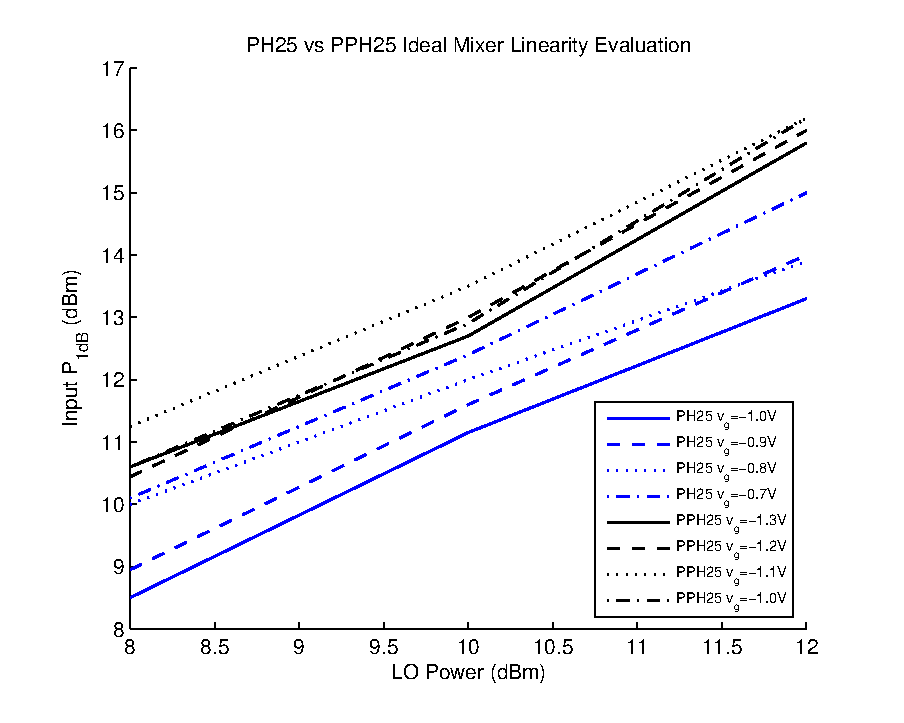
\includegraphics[width=1.0\textwidth]{fig/process/ph25vspph25}
				\caption[$P_{1dB}$ for an ideal FET resistive mixer for both PH25 and PPH25.]{$P_{1dB}$ for an ideal FET resistive mixer for both PH25 and PPH25. $P_{1dB}$ is generally \unit[1]{dB} higher for PPH25.}\label{fig:ph25vspph25}
			\end{figure}

		\subsection{Amplifier LO}
			Since neither low noise nor high power is of importance for the LO-amplifier, the choice of process has little effect.

		\subsection{Amplifier IF1}
			Amplifier IF1 does not use the amount of power that motivates the use of PPH25. The noise does however depend on the process choice. As explained in \autoref{sec:if1noise} there are no noise models for the PPH25 process. However, the noise level is through measurements estimated to be approximately \unit[0.5]{dB} higher for PPH25 than for PH25.

		\subsection{Attenuators}
			The loss in the attenuator-FETs when closed is marginally less for PPH25 than for PH25. The difference is at most \unit[0.1]{dB} per FET. As the attenuators are placed after the first amplifier, the effect of these losses is small on the total noise figure of the chip.

		\subsection{Amplifier IF2}
			The main reason for considering PPH25 is to increase the DC-power of the last amplifier (\autoref{sec:if2power}). The maximum DC current in an inductor for PH25 is merely \unit[44]{mA}.\autocite{ph25manual} The same value for PPH25 is \unit[130]{mA}.\autocite{pph25manual} The RF-choke in the bias network requires an inductor to prevent the RF-signal from escaping. A work-around for PH25 would be to create an inductor out of a long microstrip. This is however space inefficient as an inductor of this kind at \unit[2.14]{GHz} is large.

			A PH25 amplifier biased at $i_{ds}=\unit[44]{mA}$ gives $P_{1dB}\approx \unit[3]{dBm}$. The equivalent PPH25 amplifier used in the final design biased at $i_{ds}=\unit[110]{mA}$ gives $P_{1dB}\approx \unit[10]{dBm}$. Both have \unit[12]{dB} gain.

		\subsection{Summary}
			\autoref{tab:ph25vspph25} states the final performance for a system with PH25 and for a, besides the FET, equivalent system with PPH25. Estimates are made for both the extreme gain cases as well as for nominal gain. The chip design i.e. the choice and order of components is the same as the one chosen for the project (\autoref{tab:confper1}).

			\begin{table}[hbt!]
				\caption[PH25 vs PPH25 chip performance.]{Performance for PH25 and PPH25 at different gain states. Here it is assumed that $IIP_3=P_{1dB}+\unit[10]{dBm}$ for the mixer and $IIP_3=P_{1dB}+\unit[11]{dBm}$ for the amplifiers. These estimates are considered conservative.}
				\label{tab:ph25vspph25}
				\centering
				\begin{tabular}{ l l l l l l l } \toprule
					& \multicolumn{2}{c}{Nominal Gain} & \multicolumn{2}{c}{Gain: \unit[+5]{dB}} & \multicolumn{2}{c}{Gain: \unit[-5]{dB}} \\\cmidrule{2-7}
					& PH25 & PPH25 & PH25 & PPH25 & PH25 & PPH25 \\\cmidrule{2-7}
					Gain & \unit[9]{dB} & \unit[9]{dB} & $\unit[14]{dB}$ & \unit[14]{dB} & \unit[4]{dB} & \unit[4]{dB} \\
					$\nf$ & \unit[11.4]{dB} & \unit[11.8]{dB} & \unit[10.5]{dB} & \unit[11.0]{dB} & \unit[13.3]{dB} & \unit[13.6]{dB} \\
					$IIP_3$ & \unit[15.8]{dB} & \unit[19.7]{dB} & \unit[12.2]{dB} & \unit[17.7]{dBm} & \unit[18.2]{dBm} & \unit[20.6]{dBm} \\\bottomrule
				\end{tabular}
			\end{table}

	\section{Conclusion}
		From \autoref{tab:ph25vspph25} one can see that even though the PPH25 process suffers from \unit[0.5]{dB} higher noise figure, it is vastly more linear.

		%One more thing not considered in the estimates is that the microstrips in the PPH25 process may have lower resistance than those in PH25. This is because the ?? layer is thicker, which decreases the losses and thereby also reduces the noise.\autocite{??} The extent of this effect is not known. % Need to talk with Niklas about this

		For the first component in a receiver chain, where low noise is of utter importance, PH25 is the better choice. At least until the noise level in the PPH25 process can be confirmed and real noise models can be used in the design process. In this stage however, the first down-converter, the noise is not that important and the PPH25 power features makes it a better option.
